\section{Communicating Interacting Reactive Objects}
\begin{itemize}
    \item A modeling notation for reactive systems
    \item State machines
    \item Modeling cooperation
    \item Modeling of structure
\end{itemize}

\subsection{Introduction}
What is CIRO?
\begin{itemize}
    \item UML extension
    \item Notation extension for the CIP-Semantics in UML (CIP=Communicating Interacting Processes)
    \item To model reactive systems
    \item Communicating: Asynchronous communication with (event-, action-, communication-) messages
    \item Interacting: Synchronous interaction between reactive-objects
\end{itemize}
CIRO-Models
\begin{itemize}
    \item Complete description of reactive behaviour
    \item Executable model-simulation
    \item Models allow consistency and completeness checking
    \item Code-generation possible
\end{itemize}
Why extend UML?
\begin{itemize}
    \item UML is a very generic modelling language supporting software engineering in general and even more
    \item UML provides mechanisms to extend the metamodel
    \item Embedded software engineering is a specific domain of software engineering
    \item CIRO extends UML to better support the embedded domain
          \begin{itemize}
              \item Supports the proposed generic architecture
              \item Strives for decoupling
              \item Enhances component-based modelling
              \item Adds details to modelling of reactive objects and interaction between them
              \item Facilitates the development of independent component classes
              \item Adds abstractions to define interaction between components
          \end{itemize}
\end{itemize}

\subsubsection{Meta Model}
A model of model which defines
\begin{itemize}
    \item The elements of a modeling language and how they can be combined
    \item The set of potential models (syntactically correct models)
    \item The semantics (i.e. the meaning) of the model elements
\end{itemize}

\columnratio{0.5}
\begin{paracol}{2}
    \subsubsection{Component based Models}
    \begin{itemize}
        \item Configuration (or Composition): Consists of components and connectors
        \item Component
              \begin{itemize}
                  \item Independent part of a configuration
                  \item Comprises state and behaviour (UML-Object, instance of a class)
                  \item Connection-Points: Ports or implicitly, i.e. the object itself
              \end{itemize}
        \item Connectors (Links in UML)
              \begin{itemize}
                  \item Independent parts of a configuration
                  \item Define the interaction of components, i.e. if and how components can interact
                  \item Connect components via ports or directly
              \end{itemize}
    \end{itemize}
    Remarks
    \begin{itemize}
        \item In contrast to association $\rightarrow$ connectors belong to the configuration (composite) and not to the relationships originating class
        \item Components do not know the other components
        \item From the view of a component class, the interface to the outside world is given by its ports and its implicit interface (see below)
        \item Implicit interface: part of the interface defined in the component class itself, i.e. a list of operation signatures (input and output)
        \item Configurations may be used as components of a higher level
    \end{itemize}

    \switchcolumn

    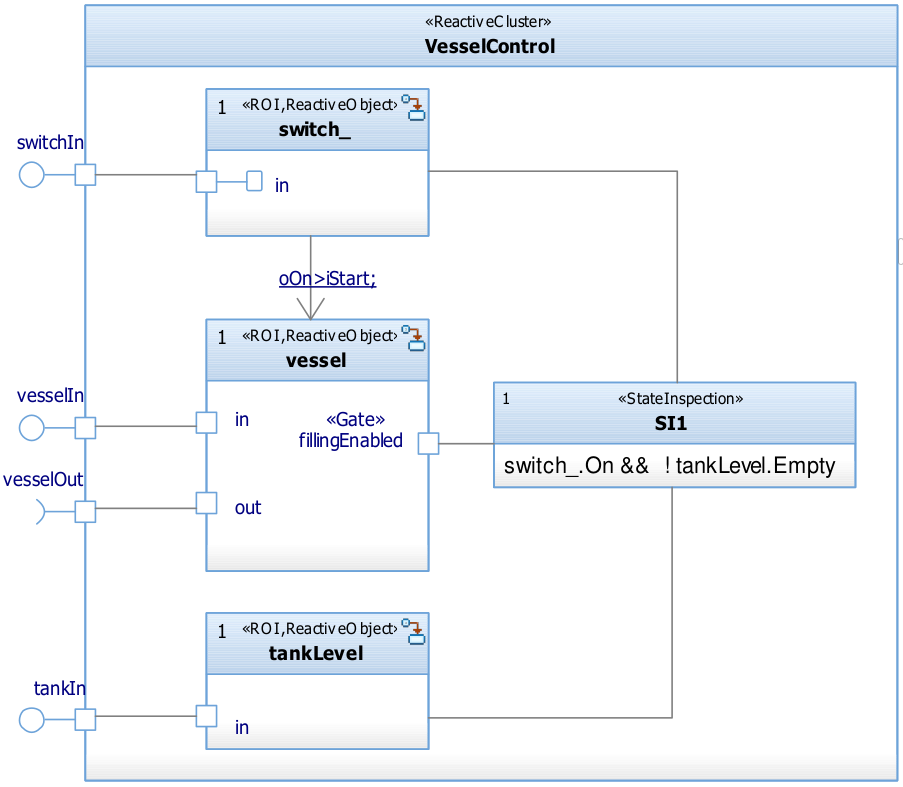
\includegraphics[width=0.49\textwidth]{images/ReactiveBehaviourNotation/component_based_model.png}
\end{paracol}

\columnratio{0.5}
\begin{paracol}{2}
    \subsection{Reactive System}
    \begin{itemize}
        \item Reactive system consists of all reactive machines of an embedded system
        \item A reactive machine is modeled as one or more reactive clusters
        \item A reactive cluster consist of cooperating state machines, i.e. reactive objects
    \end{itemize}

    \switchcolumn

    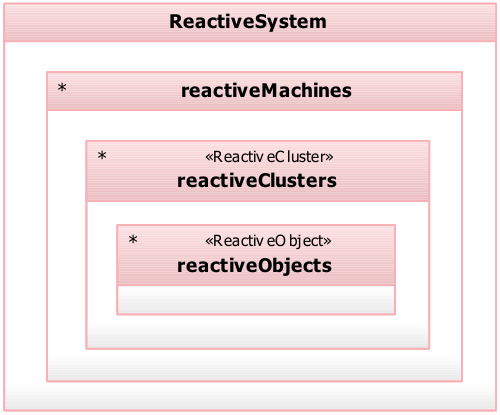
\includegraphics[width=0.35\textwidth]{images/ReactiveBehaviourNotation/reactive_system.png}
\end{paracol}
\textbf{Why multiple state machines?}
\begin{itemize}
    \item Domain orientation: Technical processes correspond to reactive objects in the model
    \item Multiple independent technical processes
          \begin{itemize}
              \item Technical system state = combination of states of technical processes
              \item State explosion
          \end{itemize}
    \item Readability of the model
    \item Division of the problem into smaller, less complex parts $\rightarrow$ \glqq divide et impera\grqq
\end{itemize}

\subsubsection{Reactive Cluster}
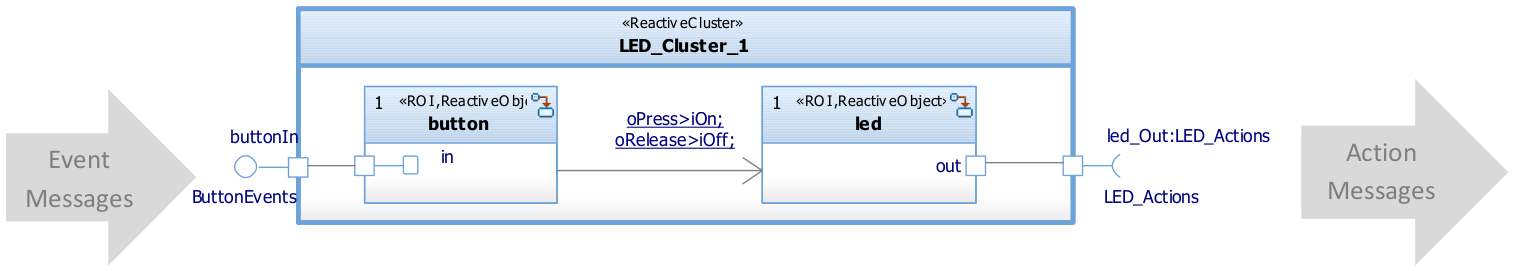
\includegraphics[width=1\textwidth]{images/ReactiveBehaviourNotation/cluster_example.png}
\begin{itemize}
    \item Part of a reactive system
    \item Reacts to event messages and generates action messages
    \item The components of a reactive cluster are reactive objects
    \item A cluster sends and receives messages via ports
    \item Ports define the interface of a cluster
    \item Within a cluster reactive objects cooperate using 3 different \textbf{synchronous} interaction mechanisms
          \begin{itemize}
              \item Pulse cast
              \item State inspection
              \item Mode control
          \end{itemize}
    \item In- and out-ports define the interface of a cluster
\end{itemize}
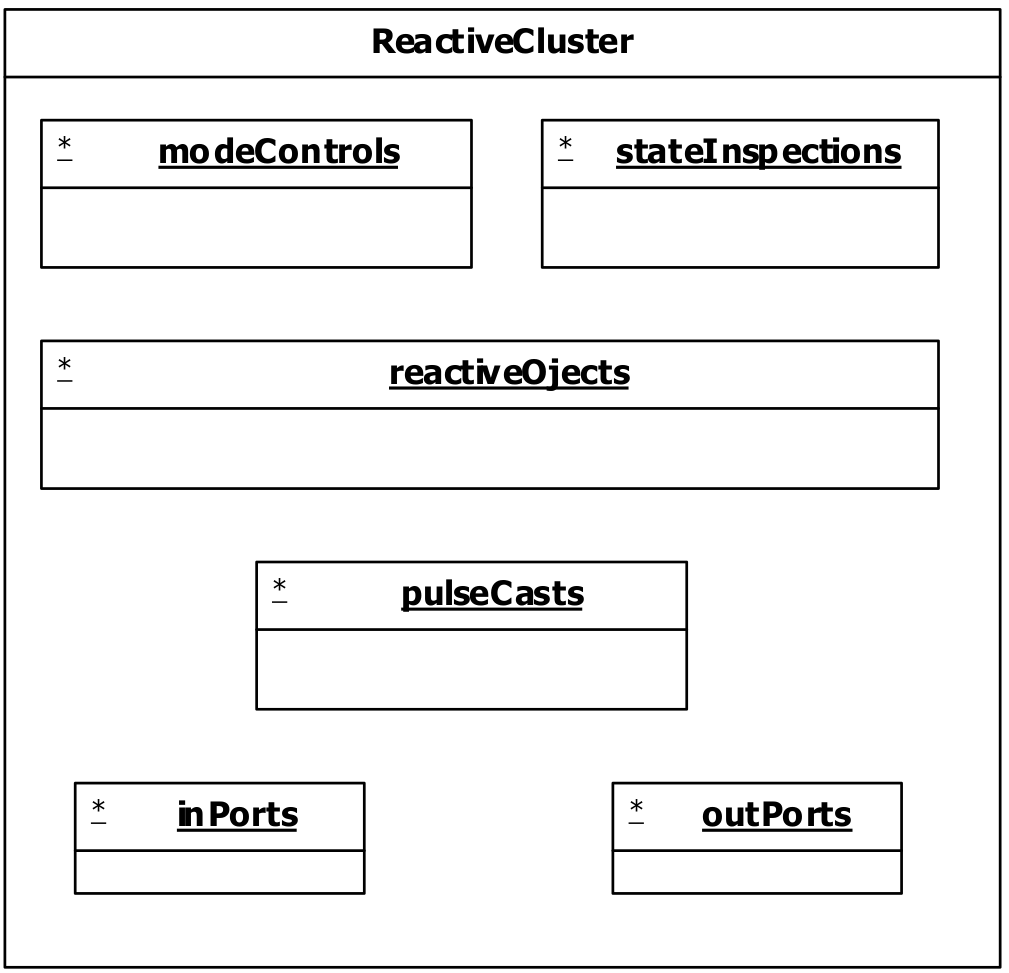
\includegraphics[width=0.4\textwidth]{images/ReactiveBehaviourNotation/meta_cluster.png}

\columnratio{0.6}
\begin{paracol}{2}
    \subsubsection{Reactive Object}
    \begin{itemize}
        \item Component of a reactive cluster
        \item The behaviour is defined by a finite state machine (FSM)
        \item The lowest reactive component in the composition hierarchy (except for composite reactive objects)
        \item Interacts synchronously with other reactive objects within the same cluster
        \item Communicates indirectly via cluster ports with the outside world by \textbf{asynchronous} messages
        \item Reactive objects are defined by a class with stereotype \texttt{<<ReactiveObject>>}
    \end{itemize}
    Behaviour / Modes
    \begin{itemize}
        \item Behaviour is defined by a state machine
        \item the state machine may be split into a number of mode state charts
        \item Each describing the behaviour of a specific operation mode
        \item All mode state charts together define the state machine of a reactive object
    \end{itemize}
    Restrictions
    \begin{itemize}
        \item Operations, attributes and parts should be private
        \item Reactive-objects should only interact by the following mechanisms with other objects: pulse-cast, state-inspection, mode-control, message passing
    \end{itemize}

    \switchcolumn

    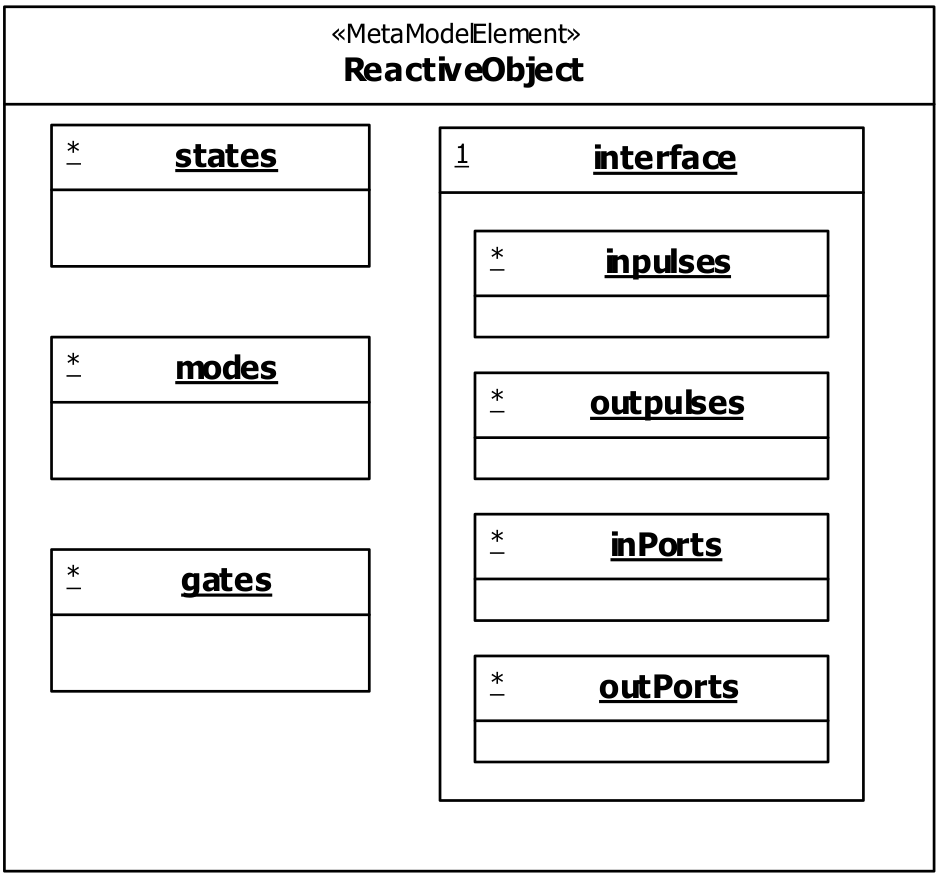
\includegraphics[width=0.39\textwidth]{images/ReactiveBehaviourNotation/meta_reactive_object.png}
\end{paracol}

\subsection{Interactions}
\begin{description}
    \item[Synchronous object interaction] $ $
          \begin{itemize}
              \item The sender or caller waits until the call is served
              \item E.g. an operation call, the caller waits until the operation returns
              \item The control-flow goes from sender to receiver
              \item The data-flow may go in both directions
                    \begin{itemize}
                        \item Parameter values are passed from sender to receiver
                        \item Return values go in the opposite direction
                    \end{itemize}
          \end{itemize}
    \item[Asynchronous object interaction]$ $
          \begin{itemize}
              \item The sender or caller proceeds immediately after the call (does not wait)
              \item The message may be stored in a buffer, e.g. a queue
              \item Data may only flow from sender to receiver
          \end{itemize}

\end{description}